\documentclass[border=10pt]{standalone}
\usepackage[svgnames]{xcolor}
\usepackage{amsmath}
\usepackage{pgfplots}
\pgfplotsset{compat=newest}
\usepackage[sfdefault]{FiraSans}
\usepackage{FiraMono}
\renewcommand*\familydefault{\sfdefault}
\begin{document}
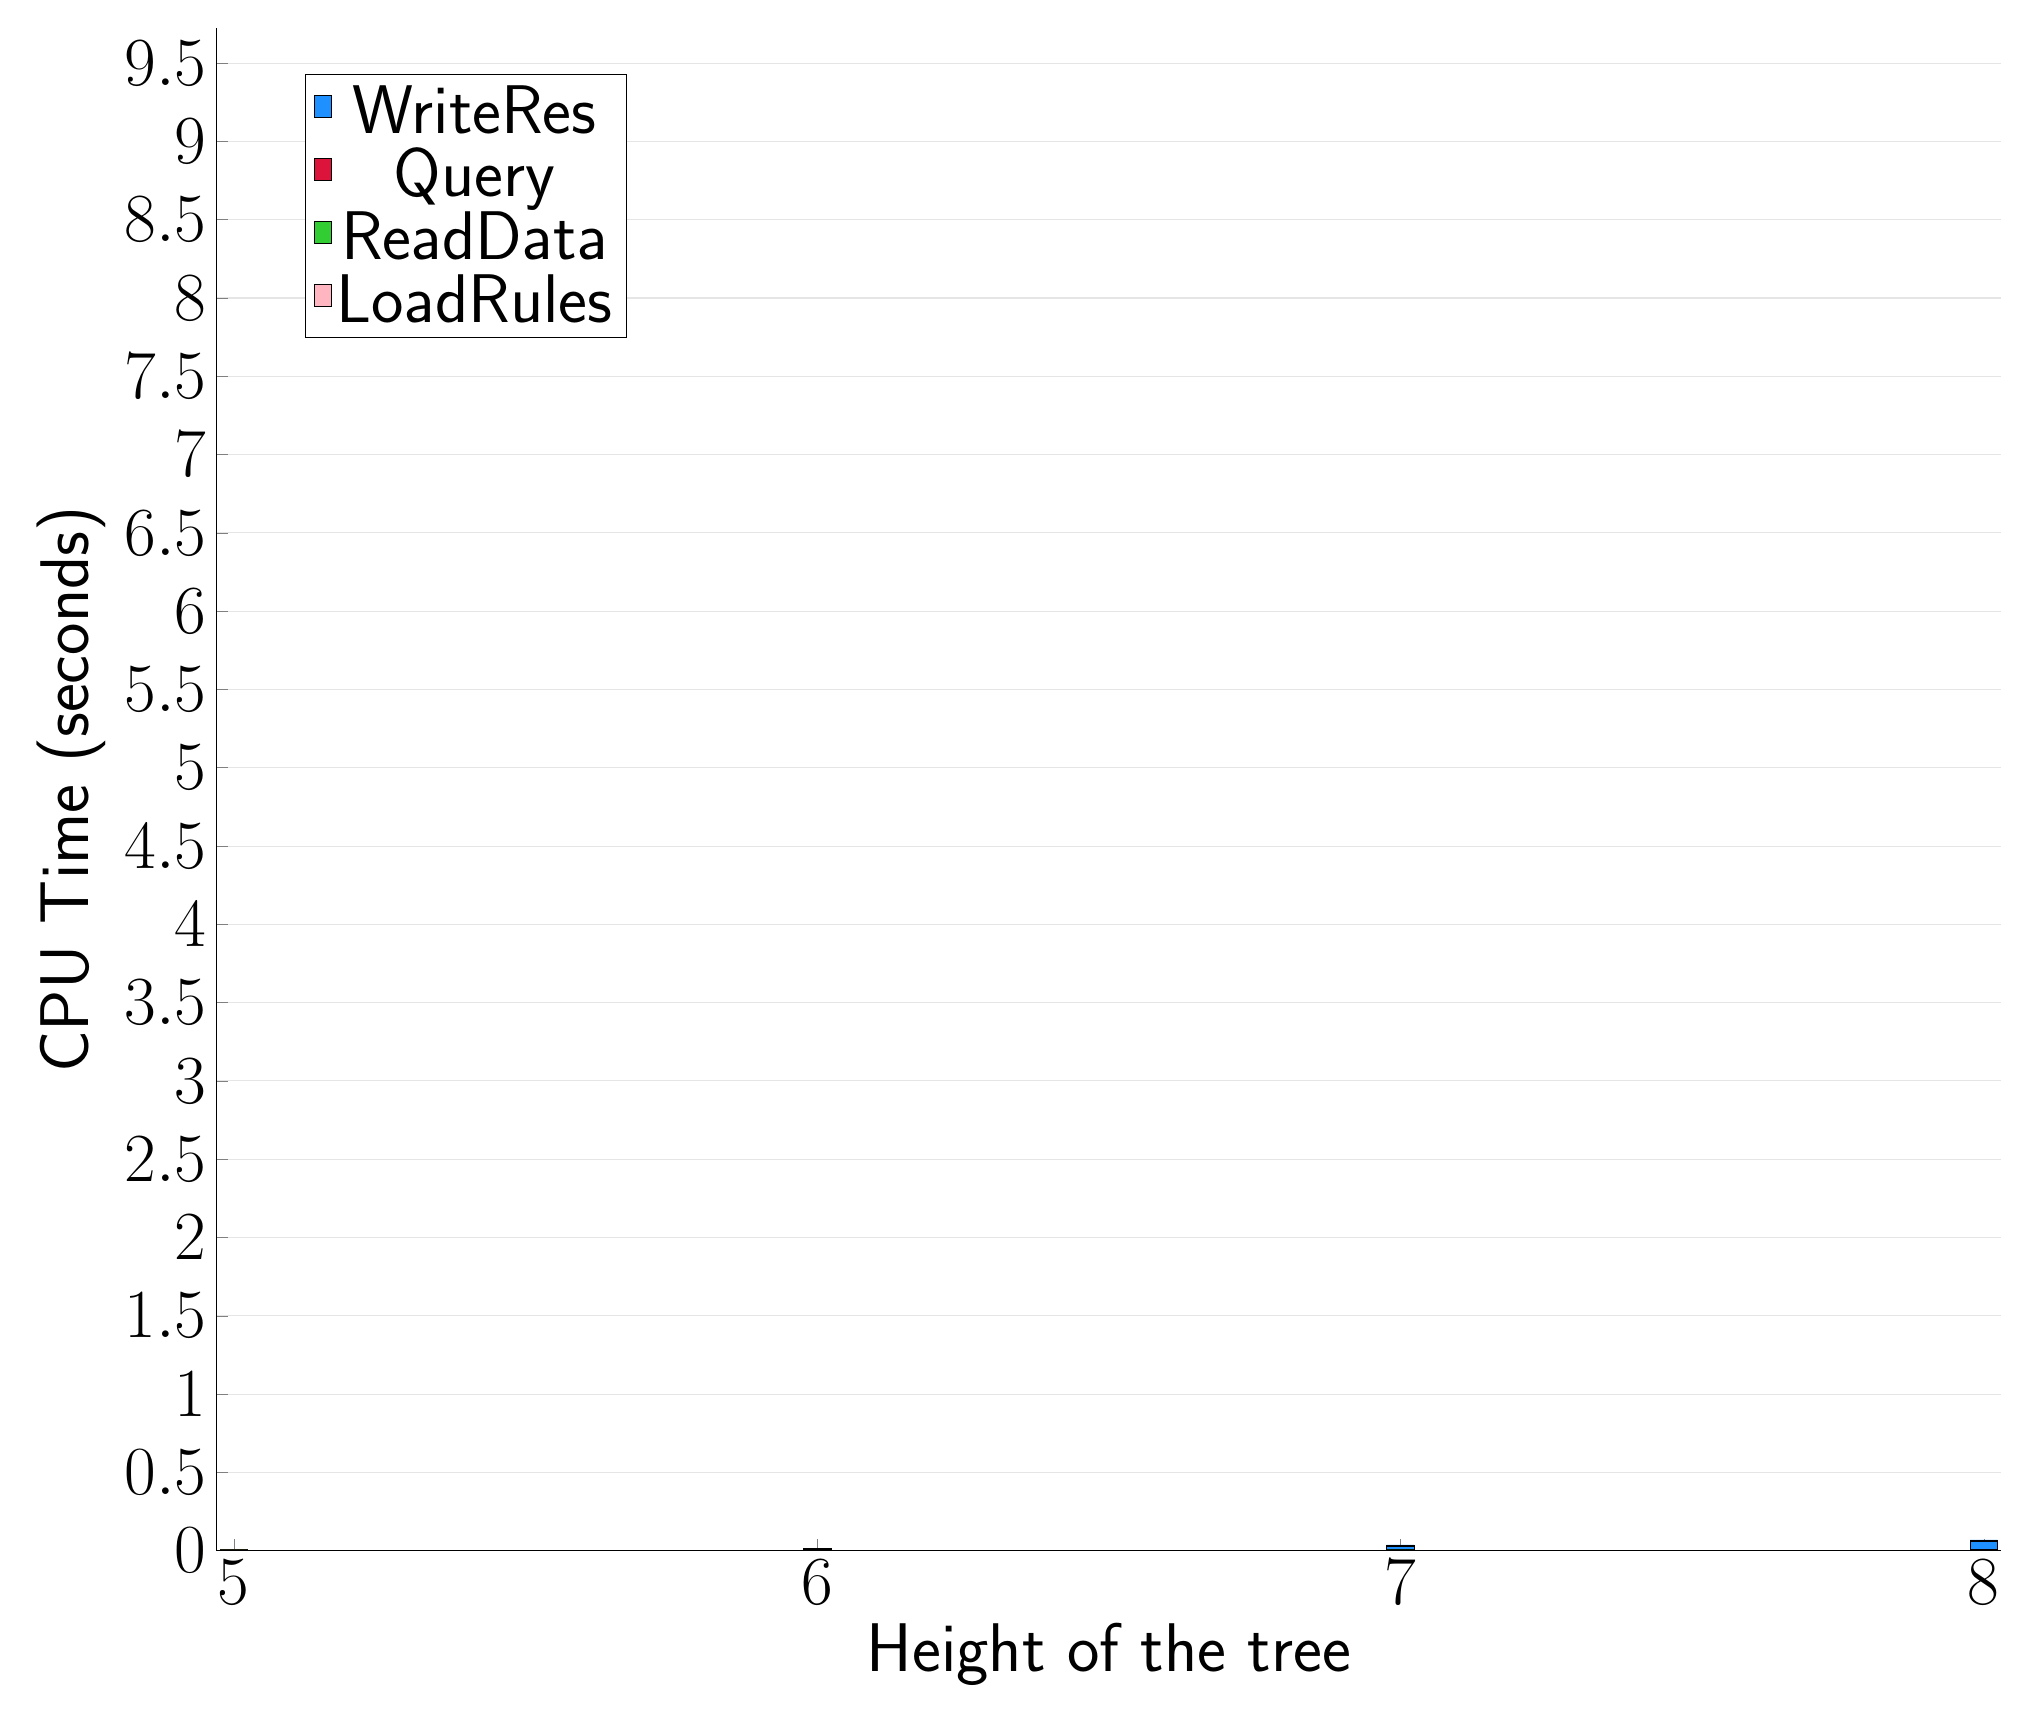
\begin{tikzpicture}
\begin{axis}[
   ybar stacked,
   width=2\textwidth,
   bar width=0.35cm,
   ymajorgrids, tick align=inside,
   major grid style={draw=gray!20},
   xtick=data,
   ymin=0, ymax=9.723333331445852,
   axis x line*=bottom,
   axis y line*=left,
   enlarge x limits=0.01,
   legend style={
       at={(0.23, 0.97)},
       anchor=north east,
       legend columns=1,
       font=\Huge,
   },
   ylabel={CPU Time (seconds)},
   xlabel={Height of the tree},
   label style={font=\Huge},
   tick label style={font=\Huge},
]
\addlegendimage{fill=DodgerBlue, draw=black, line width=0.2pt}
\addlegendentry{WriteRes}
\addlegendimage{fill=Crimson, draw=black, line width=0.2pt}
\addlegendentry{Query}
\addlegendimage{fill=LimeGreen, draw=black, line width=0.2pt}
\addlegendentry{ReadData}
\addlegendimage{fill=LightPink, draw=black, line width=0.2pt}
\addlegendentry{LoadRules}
\addplot +[fill=LightPink, draw=black, line width=0.2pt] coordinates {
(5, 0.003689666666666666)
(6, 0.004121333333333334)
(7, 0.0031739999999999997)
(7, 0.003501666666666667)
(7, 0.0028339999999999997)
(8, 0.003540666666666663)
(8, 0.0037126666666666666)
(8, 0.00379)
};
\addplot +[fill=LimeGreen, draw=black, line width=0.2pt] coordinates {
(5, 0.0012596666666666635)
(6, 0.001671333333333333)
(7, 0.002276)
(7, 0.0014449999999999999)
(7, 0.001737)
(8, 0.0040580000000000034)
(8, 0.003551666666666667)
(8, 0.0038436666666666667)
};
\addplot +[fill=Crimson, draw=black, line width=0.2pt] coordinates {
(5, 4.433333333333373e-05)
(6, 9.399999999999913e-05)
(7, 0.000176666666666668)
(7, 0.00010866666666666667)
(7, 0.000234333333333334)
(8, 0.0004226666666666663)
(8, 0.0004459999999999996)
(8, 0.00041833333333333333)
};
\addplot +[fill=DodgerBlue, draw=black, line width=0.2pt] coordinates {
(5, 0.002643999999999999)
(6, 0.009849666666666668)
(7, 0.021969)
(7, 0.031106666666666668)
(7, 0.027242000000000002)
(8, 0.061045999999999996)
(8, 0.05393333333333333)
(8, 0.05941133333333334)
};
\end{axis}
\end{tikzpicture}

\end{document}
